\section{Frontal method}
\subsection{Introduction}
\begin{exm}
    In the methods for factorization discussed earlier in this 
    chapter, we have assumed that the matrix $\mA$ is given. 
    However, the matrix is `assembled' as the sum of 
    submatrices sometimes, mostly in finite-element problems. 

    In a finite-element problem the matrix is a sum
    \begin{equation}
        \label{eq::assemble}
        \mA=\sum_l\mA^{[l]},
    \end{equation}
    where each $\mA^{[l]}$ has entries only in the principal 
    submatrix corresponding to the variables in element $l$ 
    and represents the contributions from this element. It is 
    normal to hold each $\mA^{[l]}$ in packed form as a small 
    full matrix together with a list of indices of the 
    variables that are associated with element $l$.
\end{exm}

\begin{defn}[Fully summed]
    The formation of the sum \eqref{eq::assemble} is called 
    \textit{assembly} and involves the elementary operation
    \begin{equation}
        \label{eq::elementassemble}
        a_{ij}:=a_{ij}+a_{ij}^{[l]}.
    \end{equation}
    We have used the Algol symbol ‘$:=$’ here to avoid 
    confusion with the superscript notation $a_{ij}^{(k)}$. 
    We call an entry \textit{fully summed} when all 
    contributions of the form \eqref{eq::elementassemble} have 
    been summed.
\end{defn}

\begin{lem}
    \label{lem::frontaleliminate}
    It is evident that basic operation of Gaussian elimination
    \begin{equation}
        \label{eq::frontaleliminate}
        a_{ij}^{(k+1)}=a_{ij}^{(k)}-a_{ik}^{(k)}(a_{kk}^{(k)})^
        {-1}a_{kj}^{(k)}
    \end{equation}
    may be performed before all the assemblies 
    \eqref{eq::elementassemble} are complete, provided only the 
    terms in the triple product in \eqref{eq::frontaleliminate} 
    are fully summed. Each variable can be eliminated as soon 
    as its row and column is fully summed, that is after its 
    last occurrence in a matrix $\mA^{[l]}$.
\end{lem}

\begin{defn}
    By Lemma \ref{lem::frontaleliminate}, the elimination 
    operations will be confined to the submatrix of rows and 
    columns corresponding to variables that have not yet been 
    eliminated, but are involved in one or more of the elements 
    that have been assembled. This permits all intermediate
    working to be performed in a full matrix whose size 
    increases when a variable appears for the first time and 
    decreases when one is eliminated. The pivotal order is 
    determined from the order of the assembly. If the elements 
    are ordered systematically from one end of the region to 
    the other, the active variables form a front that moves 
    along it. For this reason, the full matrix in which all 
    arithmetic is performed is called the \textit{frontal 
    matrix} and the technique is called the 
    \textit{frontal method}.
\end{defn}

\begin{exm}
    In Figure \ref{fig::Frontal}, we show the situation after 
    a set of elimination and just prior to another assembly. 
    The fully-summed rows and columns in blocks $(1,1)$, 
    $(1,2)$ and $(2,1)$ contain the corresponding rows and 
    columns of $\mL$ and $\mU$. They will not be needed until 
    the solve stage, so may be stored on auxiliary storage as
    packed vectors. Blocks $(3,1)$ and $(1,3)$ are zero 
    because the eliminated variables are fully summed. Block 
    $(2,2)$ is the frontal matrix, normally held in memory. 
    Blocks $(2,3)$, $(3,2)$, and $(3,3)$ as yet have no 
    contributions, so require no storage.
    \begin{figure}[H]
        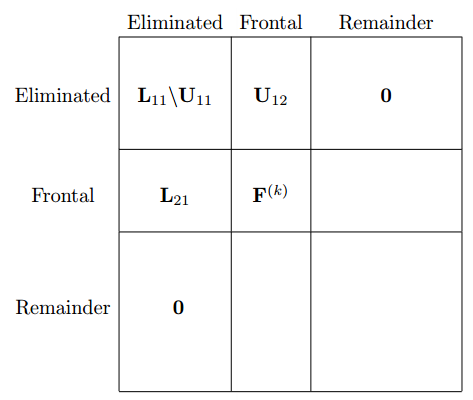
\includegraphics[width=0.8\linewidth]{png/Frontal.png}
        \caption{Matrix of partially processed frontal method}
        \label{fig::Frontal}
    \end{figure}
\end{exm}

\subsection{Element assembly tree}
In this section, we assume that the assembled matrix is 
SPD so that numerical pivoting is not 
needed for stability.
\begin{defn}
    Consider the finite-element case. The grouping of elements 
    into substructures and of substructures into bigger 
    substructures until the whole problem is obtained can be 
    expressed as a tree that is know as an \textit{element 
    assembly tree}. In an element assembly tree, each node 
    corresponds to an assembly of a frontal matrix (nothing to 
    do at a leaf node) and subsequent eliminations to form the 
    generated element matrix (also known as the `contribution 
    block').
\end{defn}

\begin{exm}
    For the finite-element problem shown on the left of Figure 
    \ref{fig::FEMproblem}, the substructure defined by nested 
    dissection can be represented by the tree shown on the 
    right of Figure \ref{fig::FEMproblem}
    \begin{figure}[H]
        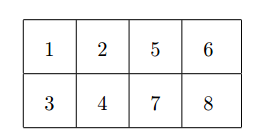
\includegraphics[width=0.45\linewidth]{png/FEMproblem.png}
        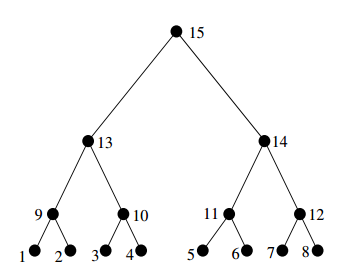
\includegraphics[width=0.45\linewidth]{png/assemblytree.png}
        \caption{A finite-element problem and the corresponding 
        element assembly tree}
        \label{fig::FEMproblem}
    \end{figure}
    This nested grouping of elements into substructures can 
    also be represented by bracketing of the sum
    \begin{align*}
        \mA=\sum_{l}\mA^{[l]}=&((\mA^{[1]}+\mA^{[2]})+
        (\mA^{[3]}+\mA^{[4]})+\\
        &(\mA^{[5]}+\mA^{[6]})+(\mA^{[7]}+\mA^{[8]})).
    \end{align*}
    For the above element assembly tree, we may perform the 
    eliminations as follows:
    \begin{enumerate}[(i)]
        \item Eliminate all variables that belong in only one 
                element, storing the resulting pivotal rows 
                and columns, and setting the resulting 
                generated element matrices aside temporarily.
        \item Assemble the resulting matrices in pairs and  
                eliminate any variable that is internal to a 
                single pair; store the resulting generated element matrices $\mA^{[9]}\sim\mA^{[12]}$.
        \item Repeat the second step until there is only one 
                structure.
    \end{enumerate}
\end{exm}

\subsection{Elimination tree}
In this section, we take as our starting point a given 
SPD matrix of order $n$.

\begin{defn}
    Just like the element assembly tree, we can construct a 
    tree called \textit{elimination tree} to arrange the 
    ordering of the elimination. It has a node for each row of 
    the matrix, if node $a$ is a child of node $b$, it means 
    that the elimination of pivot $a$ will have contribution 
    to $b$.
\end{defn}

\begin{lem}
    \label{lem::emtree}
    Suppose row $k$ has the first off-diagonal entry in the 
    column $l>k$, then row $k$ must appear ahead of row $l$ 
    since otherwise the numerical values in row $l$ when it 
    becomes pivotal will be different. We represent this by an 
    edge $(k,l)$. For any other entry $m>l$, the elimination 
    at step $k$ will fill entry $a_{lm}^{(k)}$, if not already 
    filled, so $m$ must be an ancestor of $l$ (when $m$ is 
    smaller than the first off-diagonal entry in row $l$ when 
    eliminating pivot $l$, $m$ will be the parent of $l$). By 
    this procedure, for any node $k_1$, we can get a sequence 
    of edges to nodes $k_1<k_2<...<k_r$, ending at a node 
    $k_r$ corresponding to a row that has no entries to the 
    right of the diagonal when eliminating it.
\end{lem}

\begin{exm}
    In Figure \ref{fig::emtree}, row $1$ and $2$ may be 
    interchanged without having any effect on the operations 
    performed, but row $1$ must precede row $3$. Since $3$ is 
    the first off-diagonal entry when eliminating pivot $1$, 
    it will be the parent of $1$. Since $a_{24},a_{25}\neq 0$, 
    there will be a fill-in in position $a_{45}^{(2)}$, so row 
    $4$ must precede row $5$. Since $5$ is the first 
    off-diagonal entry when eliminating pivot $4$, it will be 
    the parent of $4$. The corresponding elimination tree is 
    shown on the right of Figure \ref{fig::emtree}.
    \begin{figure}[H]
        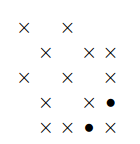
\includegraphics[width=0.45\linewidth]{png/emtree1.png}
        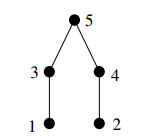
\includegraphics[width=0.45\linewidth]{png/emtree2.png}
        \caption{A matrix (each fill-in is marked as a point) 
        and the corresponding elimination 
        tree}
        \label{fig::emtree}
    \end{figure}
\end{exm}

\begin{alg}[Generate the elimination tree]
    \label{alg::emtree}
    \cite{Liu1986} has given an efficient way to generate the 
    elimination tree, essentially in time proportional to the 
    number of entries in the original matrix.

    We first consider what happens if we try to generate the
    elimination tree for a symmetric matrix that is reducible, 
    that is, a permutation of a block diagonal matrix. The 
    equations for a single block are then independent of the 
    other equations and the elimination tree for this block 
    will have as its root the node corresponding to the 
    variable in the block that is last in the pivotal order. If 
    there are $m$ blocks, there will be $m$ such elimination 
    trees, so we have a forest. So now we only consider 
    irreducible matrices.

    The $k$-th stage ($k=1,...n$) of Liu's algorithm starts 
    with the elimination forest for the leading submatrix of 
    order $k-1$, this will often be a forest rather than a tree 
    since a submatrix of an irreducible matrix may be 
    reducible. He then add the entries of column $k$ of the 
    original matrix one by one and the forest is updated to 
    correspond. He starts by adding a one node for column $k$. 
    When here comes an adding entry $a_{ik},\,i<k$, notice 
    that $k$ is the largest node for now, we will find that $k$ 
    is the parent of $i$'s root by Lemma \ref{lem::emtree}. 
    Follow this procedure until all the nonzeros in column $k$ 
    of the leading submatrix of order $k$ have been considered, 
    the forest is fully updated and we are ready to go to stage 
    $k+1$.
\end{alg}

\begin{exm}
    We show how algorithm \ref{alg::emtree} work in Figure 
    \ref{fig::algemtree}, which corresponding to updating the 
    forest during the processing of the final column of Figure 
    \ref{fig::emtree} . When we process $a_{25}$ we find that 
    node $2$ has node $4$ as its root, so there is a fill-in at 
    position $(5,4)$ so node $5$ is moved to be the parent of 
    node $4$. When we process $a_{35}$, we find that node $3$ 
    is already a root, so node $3$ is given node $5$ as its 
    parent.
    \begin{figure}[H]
        \centering
        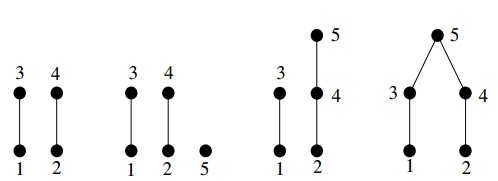
\includegraphics[width=0.8\linewidth]{png/algemtree.png}
        \caption{Updating the forest during the processing of 
        the final column of Figure \ref{fig::emtree}}
        \label{fig::algemtree}
    \end{figure}
\end{exm}

\begin{lem}
    Having constructed the elimination tree, we may use it to 
    factorize the matrix, or another matrix with the same 
    soarsity pattern. We visit the nodes in some topological 
    order (basicly from leaves to root). At each node, we add 
    together the original `elements' (nonzeros in the pivot's 
    row and column) and the generated element matrices from the
    children (if any), perform the elimination operations with 
    the packed matrix, store the calculated rows of $\mU$, and 
    hold the generated element matrix for use later.
\end{lem}

\begin{exm}
    Actually, when no pivoting is needed, frontal method can 
    be easily generalized to matrices only have symmetric 
    pattern. For example, a matrix like
    $$
    \mA=
    \begin{bmatrix}
        2&0&0&2&1\\
        0&1&-1&0&0\\
        0&-1&0&-2&0\\
        4&0&2&14&0\\
        -6&0&0&0&-2
    \end{bmatrix}.
    $$ 

    When eliminating pivot $1$, we consider the first row and 
    column, which is
    $$
    \mA_1^{(145)}=
    \begin{bmatrix}
        2&2&1\\
        4&0&0\\
        -6&0&0
    \end{bmatrix},
    $$ 
    where $(145)$ represent the nonzero indices. The eliminated matrix 
    will be
    $$
    \mathbf{F}_1^{(145)}=
    \begin{bmatrix}
        2&2&1\\
        2&-4&-2\\
        -3&6&3
    \end{bmatrix}.
    $$ 
    The generated element matrix (contribution block) is
    $$
    \mathbf{CB}_1^{(45)}=
    \begin{bmatrix}
        -4&-2\\
        6&3
    \end{bmatrix},
    $$ 
    which is also called the \textit{Schur complement}. $(45)$ 
    means the generated elements will have contribution when 
    eliminating pivots $4$ and $5$.

    Similarly, when eliminating pivot $2$,
    \begin{align*}
        &\mA_2^{(23)}=
    \begin{bmatrix}
        1&-1\\
        -1&0
    \end{bmatrix},\,
    \mathbf{F}_2^{(23)}=
    \begin{bmatrix}
        1&1\\
        -1&-1
    \end{bmatrix},\\
    &\mathbf{CB}_2^{(3)}=\begin{bmatrix}
        -1
    \end{bmatrix}.
    \end{align*}

    When eliminating pivot $3$, notice that there is a 
    generated element matrix $CB_2^{(3)}$, we add together the 
    original elements and the generated element matrix and get
    \begin{align*}
    &\mA_3^{(34)}=
    \begin{bmatrix}
        -1&-2\\
        2&0
    \end{bmatrix},\,
    \mathbf{F}_3^{(34)}=
    \begin{bmatrix}
        -1&-2\\
        -2&-4
    \end{bmatrix},\\
    &\mathbf{CB}_3^{(4)}=
    \begin{bmatrix}
        -4
    \end{bmatrix}.
    \end{align*}
    Similarly, when eliminating pivot $4$, there are generated 
    element matrices $CB_1^{(45)}$ and $CB_3^{(4)}$, so
    $$
    \mA_4^{(45)}=
    \begin{bmatrix}
        6&-2\\
        6&3
    \end{bmatrix},\,
    \mathbf{F}_4^{(45)}=
    \begin{bmatrix}
        6&-2\\
        1&5
    \end{bmatrix},\,
    \mathbf{CB}_4^{(5)}=
    \begin{bmatrix}
        5
    \end{bmatrix}.
    $$ 
    Finally, $\mA_5^{(5)}=3=\mathbf{F}_5^{(5)}$ and the 
    factorization is complete. The elimination tree is as in 
    Figure \ref{fig::exmemtree}.
    \begin{figure}[H]
        \centering
        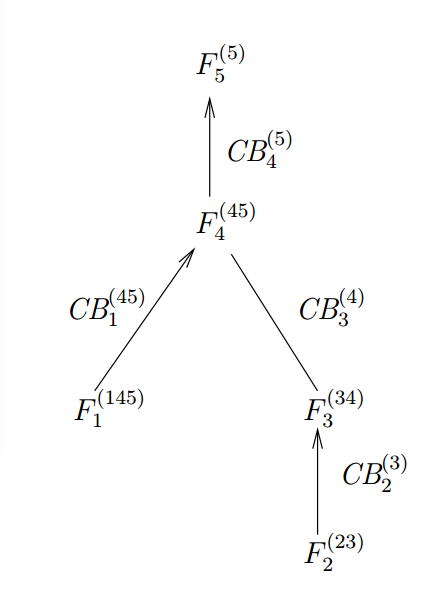
\includegraphics[width=0.5\linewidth]{png/exmemtree.png}
        \caption{Elimination tree}
        \label{fig::exmemtree}
    \end{figure}
\end{exm}

\subsection{Numerical pivoting}
\begin{alg}
    The frontal methods can also be applied to systems which 
    need numerical pivoting. As shown in Figure 
    \ref{fig::pivotfrontal}, where the block of the front 
    that is partially summed is labelled $ps$ and the parts 
    that are fully summed are labelled $fs$. Any entry whose 
    row and column is fully summed (that is, any entry in block 
    $(1,1)$ of Figure \ref{fig::pivotfrontal}) may be used as a 
    pivot. We can use any pivoting strategy including partial 
    pivoting, threshold pivoting and so on. Notice that if 
    unsymmetric interchanges are included, the index list for 
    the rows in the front will differ from columns and will 
    require separate storage.
    \begin{figure}[H]
        \centering
        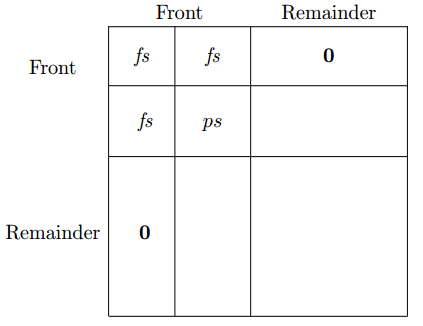
\includegraphics[width=0.8\linewidth]{png/pivotfrontal.png}
        \caption{Reduced submatrix after an assembly and prior 
        to another set of eliminations}
        \label{fig::pivotfrontal}
    \end{figure}

    It is possible that we cannot choose pivots for the whole 
    of the frontal matrix because of small entries in the front 
    or large off-diagonal entries that lie outside the block of 
    the fully-summed rows and columns (that is, because they 
    lie in block $(1,2)$ or block $(2,1)$ of Figure 
    \ref{fig::pivotfrontal}). In this case, we simply leave the
    variables in the front, continue with the next assembly, 
    and then try again. It is always possible to complete the 
    factorization using this pivotal strategy because each 
    entry eventually lies in a fully-summed row and in a 
    fully-summed column.
\end{alg}
